\documentclass[ a4paper,
                oneside,
                toc=bibliography,
                toc=listof
                ]{scrbook}

\usepackage[ngerman]{babel} % If the thesis is in English
%\usepackage[english, ngerman]{babel} % If the thesis is in German


% This class does the ISW styling for you (together with scrbook).
%
% It handles the following:
% - Proper input and font encoding (Just type, don't care about the LaTeX compiler you use or how to type German umlauts)
% - Fonts with ligatures and kerning (Tex Gyre fonts are used, part of every LaTeX installation, text is nice to read)
% - Bibliography styling for biblatex (declare your bibliography file and you are ready to go)
% - Provide command for title page (\makeISWtitle) and declaration of originality ( \declarationOfOriginality)
% - Loads packages "biblatex" and "graphics"
\usepackage[
    type=study, % master, bachelor, bachelorproject
]{iswthesis}

%Path to .bib-File(s) for BibLatex
\addbibresource{bibliography.bib}
% \addbibresource{someOtherBibFile}

\author{Lukas Schlotter}
\placeOfBirth{Stuttgart}
\major{Mechatronik}
\title{jbjhkbkj}
\titleTranslated{Wie man einen Hamster trainiert}
\matrnr{3668915}
\date{\today}
\supervisor{My supervisor, M.Sc.}
\professor{Prof. Dr.-Ing. Oliver Riedel}

\begin{document} 
    \frontmatter
    \makeISWtitle
    
    \cleardoublepage
	\setcounter{page}{1} % start at page (i) after title page
    %\declarationOfOriginality

    % Kurzfassung/Abstract
    
    \cleardoublepage
    \tableofcontents
    

    \mainmatter
    
    \chapter{Einleitung}
    Warum startet das hier mit ner 0?
    aTex allows you to manage citations within your document through the use of a separate bibtex file (filename.bib).
    
    
    \newpage
    
    Bibtex files follow a standard syntax that allow you to easily reference the citations included in that file through the use of a bibliography management package. There are multiple bibliography management packages that you can use to manage citations. \\
    This guide will demonstrate how to use biblatex which allows for the most customization.
    \section{Motivation}
    \begin{figure}[h]
    	\centering
    	
\includegraphics[width=1.0\linewidth]{./images/Test}
    	\caption{BPMN Prozess bei einem Taxiruf}
    	\label{fig:bpmn prozess}
    \end{figure}
    Dieses Bild zeigt blabla bla von dem Buch \cite{Tantau2013} und auch \cite{Kohm2013}
    
    \begin{table}[h!]
    	\centering
    	\begin{tabular}{||c c c c||} 
    		\hline
    		Col1 & Col2 & Col2 & Col3 \\ [0.5ex] 
    		\hline\hline
    		1 & 6 & 87837 & 787 \\ 
    		2 & 7 & 78 & 5415 \\
    		3 & 545 & 778 & 7507 \\
    		4 & 545 & 18744 & 7560 \\
    		5 & 88 & 788 & 6344 \\ [1ex] 
    		\hline
    	\end{tabular}
    	\caption{Table to test captions and labels.}
    	\label{table:1}
    \end{table}


	\chapter{Stand der Technik}
	
	\section{Feldbusse}
	Feldbusse: Elektrotechnik für Maschinenbauer ab S.485\\
	\\
	Feldbusse: Profibus, CAN, Sercos
	\\
	\\	
	Ethernet basierte Feldbusse: Profinet, Ethernet/IP, EtherCAT, Sercos III \\
	Ethernetbasierte Systeme sind bereit Feldbusse abzulösen \\
	\begin{figure}[!ht]
		\centering
		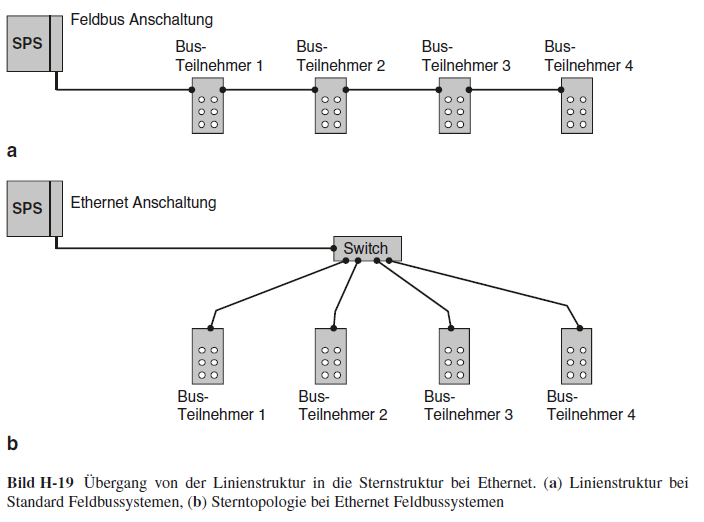
\includegraphics[width=1.0\linewidth]{./images/Feldbus vs Ethernet Anschaltung.png}
		\caption{Anschaltung Feldbus und Ethernet \cite{hering2012elektrotechnik}}
		\label{fig:Anschaltung Bus}
	\end{figure}
	\begin{figure}[!ht]
		\centering
		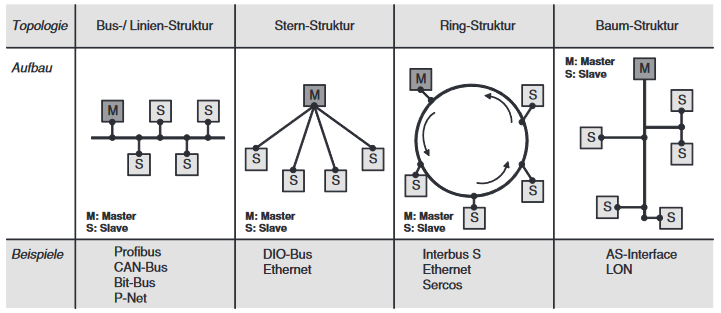
\includegraphics[width=1.0\linewidth]{./images/Topologien.png}
		\caption{Topologien}
		\label{fig:Topologien}
	\end{figure}
	Ethernet: deutlich mehr Daten als klassisch \\
	Multi-Master Bussen (z.B. CAN oder TCP/IP) vs. Mono-Master
	
	\section{TCP/IP}
   
   	MAC-Adresse eindeutig von Gerät. Für bessere Identifiuierung aber IP-Adresse
   	\begin{figure}[!ht]
   		\centering
   		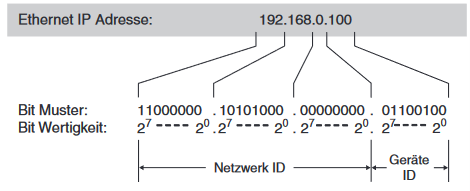
\includegraphics[width=0.70\linewidth]{./images/IP Adresse Aufbau.png}
   		\caption{Topologien}
   		\label{fig:Topologien}
   	\end{figure}
   	\\
   	Verschiedene Klassen an IP-Adressen. Meist Klasse C verwendet
   	\\
   	Weil Multi-Master-Bus braucht man CSMA/CD-Verfahren -> nicht echtzeitfähig. Lösung: Echtzeitprotokolle
   	\\
   	
	\newpage
	\chapter{Konzeptionierung}
	
	\newpage
	\chapter{Implementierung}
	
	\section{Stäubli-Roboter in VAL3}
	
	\subsection{EtherCAT}
	
	\subsection{TCP/IP}
	Für die Implementierung der TCP/IP-Verbindung auf dem Controller des Stäubli-Roboters muss in der SRS eine Socket-Verbindung angelegt werden. Hierzu wird in der E/A-Verwaltung ein Client angelegt, welcher die IP-Adresse und den Port des Servers zugewiesen bekommt. Darüber hinaus wird ein sogenannter Timeout von 0 s gesetzt. Bei einem Timeout von 0 wird auf den Vorgang, welcher ein Lesen oder Schreiben sein kann gewartet. Bei einem Timeout kleiner 0 wird hingegen nicht bis zur Ausführung des Vorgangs gewartet. Be einem Timeout größer 0 wird hingegen eine gewisse Zeit gewährt, bis zu dieser der Timeout durchgeführt werden kann. Die Nachricht soll in diesem Fall jedoch direkt gelesen oder geschrieben werden, weshalb kein Spielraum im Rahmen des Timeouts gewährt wird. \cite{VAL3} Die Socket-Verbindung wird als E/A-Verbindung in VAL3 betrachtet, weshalb eine globale Variable mit dem Namen des Clients angelegt werden kann und hierüber auch gelesen und beschrieben werden kann. Die Socket-Verbindung wird nur dann erstellt, wenn sie ihm Rahmen des Programmablaufs z.B. durch die Befehle sioSet und sioGet benötigt wird. Der Client versucht dann eine Verbindung zum Server aufzubauen.   usepackage{ffcode}\\
	num sioGet(sio siInput, num\& nData[])\\
	Diese Funktion schreibt ein gelesenes Zeichen oder einen gelesen Array von Zeichen von siInput in das Array nData. Als Rückgabewert dient die Anzahl der gelesenen Zeichen.	
	num sioSet(sio siOutput, num\& nData[]) \\
	Mit dieser Funktion kann in VAL3 die zu übermittelnde Nachricht nData versendet werden, indem der E/A-Verbindung siOutput die Nachricht zugewiesen wird. Zurückgegeben wird die Anzahl der geschriebenen Zeichen oder "-1" im Falle des Timeouts. \\
	Das Versenden von Nachrichten erfolgt über einen Byte-Array, das heißt durch die Aneinanderreihung mehrerer Bytes. Folglich muss die zu versendete Nachricht in einen Byte-Array umgewandelt werden und beim Empfangen muss der Byte-Array interpretiert werden.\\
	num toBinary(num nValue[], num nValueSize, string sDataFormat, num\& nDataByte[])\\
	Diese Funktion wandelt einen numerischen Wert, welcher das Datenformat sDataFormat besitzt in einen Byte-Strom und speichert diesen im Array nDataByte. Über das Datenformat wird beispielsweise angegeben ob es sich um einen Gleitkommawert handelt, ob ein Vorzeichen vorliegt und ob das Little-Endian oder das Big-Endian-Format angewandt wird. Mit nDataSize kann die Anzahl der zu kodierenden Zeichen beschränkt werden.\\
	num fromBinary(num nDataByte[], num nDataSize, string sDataFormat, num\& nValue[])\\
	Umgekehrt ermöglicht diese Funktion, einen empfangen Byte-Array in numerische Werte zu konvertieren. Das Ergebnis im Datenformat nDataFormat wird in nValue gespeichert. Die Anzahl der zu decodierenden Bytes wird festgelegt durch nDataSize, wenn nicht alle Bytes des Eingangs-Array nDataByte decodiert werden sollen.
	
	
	
	
   	
   	
   	\backmatter
   	
   	
   	\cleardoublepage
   	\listoffigures
   	\cleardoublepage
   	\listoftables
   	\cleardoublepage
   	
   	\cleardoublepage
   	\printbibliography
   	% Acronyms
   	
   	% Appendix, if needed:
   

\end{document}